% This is samplepaper.tex, a sample chapter demonstrating the
% LLNCS macro package for Springer Computer Science proceedings;
% Version 2.21 of 2022/01/12
%
\documentclass[runningheads]{llncs}
%
\usepackage[T1]{fontenc}
% T1 fonts will be used to generate the final print and online PDFs,
% so please use T1 fonts in your manuscript whenever possible.
% Other font encondings may result in incorrect characters.
%
\usepackage{graphicx}
% Used for displaying a sample figure. If possible, figure files should
% be included in EPS format.
%
% If you use the hyperref package, please uncomment the following two lines
% to display URLs in blue roman font according to Springer's eBook style:
%\usepackage{color}
%\renewcommand\UrlFont{\color{blue}\rmfamily}
%\urlstyle{rm}
%

\usepackage{amsmath}
\usepackage{amssymb}
\begin{document}
%
\title{Emotional Models: Supervised vs. Zero-Shot Classification}
%
%\titlerunning{Abbreviated paper title}
% If the paper title is too long for the running head, you can set
% an abbreviated paper title here
%
\author{Miguel Castela\inst{1} \and
Miguel Martins\inst{2}} 
%
\authorrunning{F. Author et al.}
% First names are abbreviated in the running head.
% If there are more than two authors, 'et al.' is used.
%
\institute{Univsersity of Coimbra, Portugal \\
\email{uc2022212972@student.uc.pt}\\
\email{uc2022213951@student.uc.pt}
}
%
\maketitle              % typeset the header of the contribution
%
\section{Introduction}

The core task addressed in this work is multi-class emotion classification. Formally, given an input text sequence $x$ (e.g., a tweet or a short message), the goal is to map $x$ to a single label $y$ from a predefined set of discrete emotions $E = \{ \text{anger, fear, joy, love, sadness, surprise} \}$.

This task presents several challenges typical of processing short, informal text. First, the limited length of the input results in sparse feature representations when using traditional bag-of-words methods. Second, the expression of emotion is often subtle and context-dependent, relying on sarcasm, negation, or idiomatic expressions that are difficult to capture without deep semantic understanding.

We approach this problem using the \texttt{dair-ai/emotion} dataset. The objective is to maximize the classification accuracy and the Macro-F1 score, the latter being particularly important to account for potential class imbalances among the six emotion categories. We contrast two distinct paradigms to solve this: a supervised approach relying on fixed embeddings and a zero-shot approach relying on natural language inference.

\section{Methodology}

To address the problem statement, we implement two parallel pipelines. Both leverage the Transformer architecture but utilize it in fundamentally different ways.

\subsection{Supervised Learning: Feature Extraction}
In the first approach, we treat a pretrained Transformer model as a feature extractor. The architecture consists of two components:
\begin{itemize}
    \item \textbf{Backbone:} A pretrained model (e.g., RoBERTa or DistilBERT) from the \texttt{sentence-transformers} library. We process the input text $x$ to obtain a dense vector representation $v \in \mathbb{R}^d$, where $d$ is the embedding dimension. The weights of this backbone are frozen during training.
    \item \textbf{Classifier Head:} A lightweight supervised model (e.g., Logistic Regression or a Multi-Layer Perceptron) trained on the pair $(v, y)$. This head learns to map the semantic embedding to the specific emotion logits.
\end{itemize}
This method mirrors the "transfer learning" workflow common in computer vision, allowing us to leverage the massive pretraining of the Transformer while keeping the training cost low.

\subsection{Zero-Shot Classification}
The second approach utilizes a Zero-Shot classification paradigm based on Natural Language Inference (NLI). Instead of training a classifier on the specific emotion labels, we use a model pretrained on NLI tasks (determining if a hypothesis contradicts, entails, or is neutral to a premise).

For each input text $x$, we construct a set of hypotheses $H = \{ h_1, \dots, h_6 \}$ using a template such as "This text expresses \textit{<emotion>}". The model computes the entailment probability $P(h_i | x)$ for each emotion. The predicted label is the emotion corresponding to the hypothesis with the highest probability:
$$ \hat{y} = \operatorname*{argmax}_{e \in E} P(\text{"This text expresses } e \text{"} \mid x) $$
This method requires no training on the \texttt{dair-ai/emotion} dataset, testing the model's ability to generalize to unseen classes purely based on their semantic description.


Subsequent paragraphs, however, are indented.

\subsubsection{Sample Heading (Third Level)} Only two levels of
headings should be numbered. Lower level headings remain unnumbered;
they are formatted as run-in headings.

\paragraph{Sample Heading (Fourth Level)}
The contribution should contain no more than four levels of
headings. Table~\ref{tab1} gives a summary of all heading levels.

\begin{table}
\caption{Table captions should be placed above the
tables.}\label{tab1}
\begin{tabular}{|l|l|l|}
\hline
Heading level &  Example & Font size and style\\
\hline
Title (centered) &  {\Large\bfseries Lecture Notes} & 14 point, bold\\
1st-level heading &  {\large\bfseries 1 Introduction} & 12 point, bold\\
2nd-level heading & {\bfseries 2.1 Printing Area} & 10 point, bold\\
3rd-level heading & {\bfseries Run-in Heading in Bold.} Text follows & 10 point, bold\\
4th-level heading & {\itshape Lowest Level Heading.} Text follows & 10 point, italic\\
\hline
\end{tabular}
\end{table}


\noindent Displayed equations are centered and set on a separate
line.
\begin{equation}
x + y = z
\end{equation}
Please try to avoid rasterized images for line-art diagrams and
schemas. Whenever possible, use vector graphics instead (see
Fig.~\ref{fig1}).

\begin{figure}
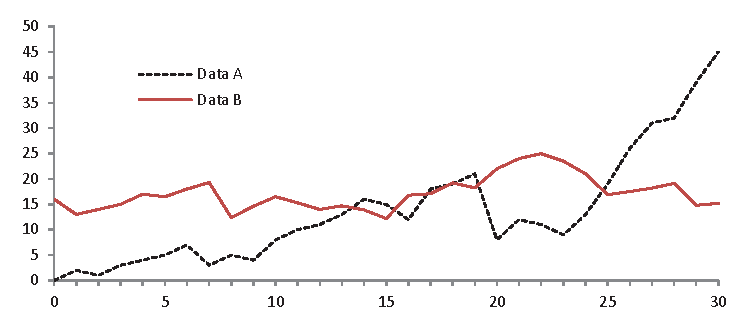
\includegraphics[width=\textwidth]{fig1.eps}
\caption{A figure caption is always placed below the illustration.
Please note that short captions are centered, while long ones are
justified by the macro package automatically.} \label{fig1}
\end{figure}

\begin{theorem}
This is a sample theorem. The run-in heading is set in bold, while
the following text appears in italics. Definitions, lemmas,
propositions, and corollaries are styled the same way.
\end{theorem}
%
% the environments 'definition', 'lemma', 'proposition', 'corollary',
% 'remark', and 'example' are defined in the LLNCS documentclass as well.
%
\begin{proof}
Proofs, examples, and remarks have the initial word in italics,
while the following text appears in normal font.
\end{proof}
For citations of references, we prefer the use of square brackets
and consecutive numbers. Citations using labels or the author/year
convention are also acceptable. The following bibliography provides
a sample reference list with entries for journal
articles~\cite{ref_article1}, an LNCS chapter~\cite{ref_lncs1}, a
book~\cite{ref_book1}, proceedings without editors~\cite{ref_proc1},
and a homepage~\cite{ref_url1}. Multiple citations are grouped
\cite{ref_article1,ref_lncs1,ref_book1},
\cite{ref_article1,ref_book1,ref_proc1,ref_url1}.

\begin{credits}
\subsubsection{\ackname} A bold run-in heading in small font size at the end of the paper is
used for general acknowledgments, for example: This study was funded
by X (grant number Y).

\subsubsection{\discintname}
It is now necessary to declare any competing interests or to specifically
state that the authors have no competing interests. Please place the
statement with a bold run-in heading in small font size beneath the
(optional) acknowledgments\footnote{If EquinOCS, our proceedings submission
system, is used, then the disclaimer can be provided directly in the system.},
for example: The authors have no competing interests to declare that are
relevant to the content of this article. Or: Author A has received research
grants from Company W. Author B has received a speaker honorarium from
Company X and owns stock in Company Y. Author C is a member of committee Z.
\end{credits}
%
% ---- Bibliography ----
%
% BibTeX users should specify bibliography style 'splncs04'.
% References will then be sorted and formatted in the correct style.
%
% \bibliographystyle{splncs04}
% \bibliography{mybibliography}
%
\begin{thebibliography}{8}
\bibitem{ref_article1}
Author, F.: Article title. Journal \textbf{2}(5), 99--110 (2016)

\bibitem{ref_lncs1}
Author, F., Author, S.: Title of a proceedings paper. In: Editor,
F., Editor, S. (eds.) CONFERENCE 2016, LNCS, vol. 9999, pp. 1--13.
Springer, Heidelberg (2016). \doi{10.10007/1234567890}

\bibitem{ref_book1}
Author, F., Author, S., Author, T.: Book title. 2nd edn. Publisher,
Location (1999)

\bibitem{ref_proc1}
Author, A.-B.: Contribution title. In: 9th International Proceedings
on Proceedings, pp. 1--2. Publisher, Location (2010)

\bibitem{ref_url1}
LNCS Homepage, \url{http://www.springer.com/lncs}, last accessed 2023/10/25
\end{thebibliography}
\end{document}
